% \documentclass[serif]{beamer} % Serif for Computer Modern math font.
\documentclass{beamer} % Handout mode to ignore pause statements
\hypersetup{colorlinks,linkcolor=,urlcolor=red}
\setbeamertemplate{navigation symbols}{} % Supress navigation symbols
\usetheme{Berlin} % Displays sections on top
\usepackage[english]{babel}
\usepackage[normalem]{ulem}
\usepackage[makeroom,thicklines]{cancel}
\usepackage{natbib}
\usepackage{hyperref}
\hypersetup{colorlinks,linkcolor={blue},citecolor={blue},urlcolor={red}}  
\newcommand{\mb}[1]{\boldsymbol{#1}}
\newcommand{\bracevec}[1]{\left\lbrace #1 \right\rbrace}

% \definecolor{links}{HTML}{2A1B81}
% \definecolor{links}{red}

\setbeamertemplate{footline}[frame number] 

\mode<presentation>
% \mode<handout>{\setbeamercolor{background canvas}{bg=black!5}}






\def\[#1\]{\begin{equation}\begin{aligned}#1\end{aligned}\end{equation}}
\def\*[#1\]{\begin{align*}#1\end{align*}}

\title{Approximate Bayesian Inference for Cox Proportional Hazard Model}
\author{Ziang Zhang, Alex Stringer, Patrick Brown, Jamie Stafford}
\institute{Department of Statistics, University of Toronto}
\date{2020-05-06}

\setbeamercovered{transparent}

\begin{document}

\begin{frame}
\titlepage
\end{frame}

\begin{frame}
\frametitle{Outline}
\tableofcontents
\end{frame}

\section{Introduction and Motivation}
\subsection{Survival Analysis}
\begin{frame}
\begin{block}{What is Survival Analysis?}
Survival analysis refers to situations in which the response variable of interest is the time until the occurrence of a particular event.
\end{block}
\pause

$\textbf{For instances: }$
\pause

Time until death of patient with a specific disease, 

\pause
Time to failure of a kind of light-bulbs, 
\end{frame}

\begin{frame}
\begin{Example}
We collect the information of 10 people (each with two kidneys) who have recovered from kidney infections such as gender, age, and type of infection on each kidney, and then record the recurrence times to infection of each kidney of each person. The study is one year long, and we hope to know whether a certain type of infection tend to recur faster conditional on the gender and age of patients.
\end{Example}
\end{frame}

\begin{frame}
\begin{enumerate}
\item Why don't we just do a linear regression? 
\pause 

$\textbf{Reason}$: The response variable is not closed to normal. It is a positive random variable with possibly very skewed distribution (for example, exponential distribution).

\pause 
\item Then why don't we just do a generalized linear regression instead?

\pause 
$\textbf{Reason}$: The exact realization of the response variable could be right-censored, so we don't know its exact value but only a lower bound for it. For example, the subject could be lost in the middle of the study, or the event never occur in the duration of the study.

\end{enumerate}
\end{frame}

\begin{frame}
Let $Y_i$ denote the i-th response variable, with pdf $f(t)$ and cdf $F(t)$. Let $y_i$ denote its realization or its censoring time. 
\pause 
\newline

Let $\delta_i$ is an indicator of whether the i-th observation is right-censored or not, so $\delta_i = 1$  means it is not right-censored so $Y_i = y_i$, and $\delta_i = 0$  means it is right-censored so $Y_i > y_i$.
\pause 
\newline

In survival analysis, we have $\{(y_i,\delta_i)|i = 1, ..., n\}$ as our data for the response variable.
\end{frame}

\begin{frame}
\frametitle{Two additional Definitions}
\begin{definition}
Survival function of $Y$ at time $t$ is defined as:
\newline

\centering
$S(t) = 1- F(t) = \text{P}(Y\geq t)$
\end{definition}

\pause

\begin{definition}
Hazard function of $Y$ at time $t$ is defined as:
\newline

\centering
$h(t) = \lim_{s\to 0} \frac{\text{P}(t\le Y \le t+s |Y\ge t)}{s} = \frac{f(t)}{S(t)}$
\end{definition}

\end{frame}

\subsection{Cox Proportional Hazard Model}
\begin{frame}

\begin{definition}
The Cox Proportional Hazard Model specifies the hazard function of the i-th observation $Y_i$ as:
\newline
\centering
$h_{i}(t) = h_{0}(t) \text{exp}(\eta_i)$
\end{definition}
\pause
Here the $\eta_i$ is the i-th additive linear predictor, for example: it could be $\beta_1\text{age}_i + \beta_2\text{sex}_i$ for a model with just two fixed effects. \newline
\pause
\newline
The component $h_{0}(t)$ is a "universal" baseline hazard function that is the $\textbf{same}$ for all the observations in our data set, but with an unspecified structure.\newline
\pause
\newline
The main interest is for inference on components of $\eta_i$, because knowing those $\beta$s is enough for us to know the relative risk of one subject to another. The baseline hazard function $h_{0}(t)$ is often of secondary interest.


\end{frame}

\subsection{Partial likelihood function}
\begin{frame}
Note that the full-likelihood of CoxPH Model is:

\begin{equation}\begin{aligned}\label{eqn:full_likelihood}
L(y|\eta) &= \prod_{i=1}^{n} h_{i}(y_i)^{\delta_i}S_{i}(y_i) \\
&= \prod_{i=1}^{n} (h_{0}(y_i) \text{exp}(\eta_i))^{\delta_i}S_{i}(y_i)
\end{aligned}\end{equation}
\pause
To actually evaluate it, we need to know what function that $h_{0}(t)$ is, which unfortunately is rare in practice...
\end{frame}

\begin{frame}

Partial likelihood of CoxPH Model can be viewed as a marginal likelihood for "observed ranks", and it doesn't require us to specify a baseline hazard function $h_{0}(t)$.\newline
\pause
Denote the risk set of observation i as : $R_i := \big\{j \in 1:n | y_j \geq y_i\big\}$, the partial likelihood can be written as: \newline
\pause
\begin{equation}\begin{aligned}\label{eqn:partial}
L(y|\eta) &= \prod_{i=1}^{n} \bigg\{\frac{h_{i}(y_i)}{{\sum_{j\in R_{i}}^{}h_{j}(y_i)}}\bigg \}^{\delta_{i}} \\
&= \prod_{i=1}^{n}\bigg\{\frac{\exp[\eta_{i}]}{{\sum_{j\in R_{i}}^{}\exp[\eta_{j}]}}\bigg \}^{\delta_{i}}\\
\end{aligned}\end{equation}
\pause
Note that the baseline hazard function $h_{0}(t)$ is cancelled out.


\end{frame}
\subsection{Motivations of Proposed Method}
\begin{frame}
$\textbf{Question}$: What if we are interested in Bayesian Inference of Cox Proportional Hazard Model?
\begin{itemize}
\pause
\item INLA with some extra conditions \citep{inlacoxph}.
\begin{itemize}
\pause
\item Can do approximate Bayesian inference on CoxPH model with the full likelihood.
\pause
\item It does not support the use of partial likelihood. To use the full likelihood, it approximates the baseline hazard function $h_{0}(t)$ with piece-wise constant functions, which may not work well when $h_{0}(t)$ is very complicated.
\end{itemize}
\pause
\item Approximate Bayesian Inference for Case-crossover Model \citep{casecross}.
\begin{itemize}
\pause
\item It does support the use of partial likelihood in its inference.
\pause
\item It can only do the inference for case-crossover model. The partial likelihood of case-crossover model has similar form with Cox PH model, but is simpler than Cox PH model in general.
\end{itemize}
\end{itemize}
\end{frame}

\section{Models and Methodology}
\subsection{Revisit of the Models}
\begin{frame}
Let's have a brief revisit of the general Cox Proportional Hazard Model (with some small modifications):
\begin{center}
$h_{i}(t) = h_{0}(t) \text{exp}(\eta_i)$
\end{center}
where the additive linear predictor $\eta_i$ can be generally defined as:
\begin{center}
$\eta_i = x_{i} ^ {T}  \beta + \gamma(u_i) + \epsilon_i$ 
\end{center}
\begin{itemize}
\pause
\item $x$ is a vector of fixed effect covariates.
\pause
\item $u$ is the smoothing covariate, and $\gamma$ is its corresponding smoothing function that we want to make inference on.
\pause
\item $\epsilon_i  \stackrel{iid}{\sim} \text{N}(0,\tau^{-1})$ is an auxiliary variable to make the computation easier, and $\tau^{-1}$ is very small.
\end{itemize}
\pause
Unlike the case-crossover model, it is also possible to include a random intercepts for each subject, which is called "frailty" between subjects in survival analysis because of the form of its partial likelihood \citep{frailty}.
\end{frame}

\subsection{Smoothing effect}
\begin{frame}
For the inference of smoothing function, we implemented second-order random walk model \citep{rw2}\newline
\begin{itemize}
\pause
\item The smoothing covariate $u$ is first discretized into $m$ disjoint bins : $\{[a_{1}, a_{2}], [a_{2}, a_{3}]...., [a_{m}, a_{m+1}] \}$. Denote the meddle points of these bins as $\{u_{1}, ..., u_{m} \}$.
\pause
\item Assume the smoothing function $\gamma$ is piece-wise constant within each bin, so the inference on $\gamma$ becomes inference on $\Gamma = \{\gamma(u_{1}),\gamma(u_{2}), ...,  \gamma(u_{m})\}$.
\pause
\item Put a second-order random walk prior on $\Gamma$, so $(\gamma(u_{i+1})-\gamma(u_{i})) - (\gamma(u_{i})-\gamma(u_{i-1})) = \gamma(u_{i-1})-2\gamma(u_{i}) + \gamma(u_{i+1}) \stackrel{iid}{\sim} \text{N}(0,\sigma_{u})$
\end{itemize}
\end{frame}

\subsection{Approximation Method}

\begin{frame}
Then, also put a joint Gaussian prior on $\beta$ such that: $\beta \sim \text{N}(0,\Sigma_{\beta})$.\newline
Let $W = (\beta, \Gamma, \eta)$, then by construction, $W$ follows a joint Gaussian as well. \newline
The hyper-parameter $\theta$ is defined as $-2\text{log}(\sigma_u)$, which controls the level of smoothness. The prior put on this is not necessary Gaussian.\newline
\end{frame}


\begin{frame}
For the approximation method, we adopt the inferential methodology of \citet{casecross}. \newline
The objects of inferential interest are the posteriors:\newline
\begin{equation}\begin{aligned}\label{eqn:approximation}
\pi(W_{j}|\mb{Y}) &= \int\int\pi(\mb{W}|\mb{Y},\theta)\pi(\theta|\mb{Y})d\mb{W}_{-j}d\theta, \\
\pi(\theta|\mb{Y}) &= \frac{\int\pi(\mb{W},\theta,\mb{Y})d\mb{W}}{\int\pi(\mb{W},\theta,\mb{Y})d\mb{W}d\theta}
\end{aligned}\end{equation}
\pause
\begin{enumerate}
\item Approximate $\pi(\theta^{k}|\mb{Y})\approx\tilde{\pi}_{LA}(\theta^{k}|\mb{Y})$, a \textbf{Laplace approximation} \citep{tierney},
\pause
\item Approximate $\pi(\mb{W}|\mb{Y},\theta^{k}) \approx \tilde{\pi}_{G}(\mb{W}|\mb{Y},\theta^{k})$, a \textbf{Gaussian approximation}. This also gives a univariate Gaussian approximation $\tilde{\pi}_{G}(W_{j}|\mb{Y},\theta^{k}) = \int\tilde{\pi}_{G}(\mb{W}|\mb{Y},\theta^{k})d\mb{W}_{-j}$.
\end{enumerate}
\pause
Choose a $\textbf{grid}$ and corresponding weights $\bracevec{\theta^{k},\Delta^{k}:k\in[K]}$. 
Then approximate $\pi(W_{j}|\mb{Y}) \approx \sum_{k=1}^{K}\tilde{\pi}_{G}(W_{j}|\mb{Y},\theta^{k})\tilde{\pi}_{LA}(\theta^{k}|\mb{Y})\Delta^{k}$.
\end{frame}

\begin{frame}
The approximation methodology is \textbf{fast} for data set with small to medium size.
\pause

The \textbf{Gaussian approximation} requires repeated high-dimensional optimizations. The objective function is \textbf{convex} but has a \textbf{dense Hessian}, so we use \textbf{trust region} optimization with \textbf{quasi-Newton method} \citep{trustoptim} to do this \textbf{fast} and \textbf{stable}.

\pause

The quasi Newton method (SR1: Symmetric Rank One) \textbf{avoids} the evaluation of the actual Hessian matrix \textbf{in each iteration of the optimization}, and therefore reduces the computational complexity during the optimization. But we still \textbf{need} the value of the Hessian matrix \textbf{at each optimal points} for the approximation.

\pause

The computations which need to be done for multiple $\theta^{k}$ are done in \textbf{parallel}.
\end{frame}

\section{Applications and Results}
\subsection{Simulation Study}
\begin{frame}
To show the accuracy of our approach compared to INLA when the baseline hazard function is non-smooth, we did the following simulation:
\begin{itemize}
\item We simulate $\textbf{N} = 400$ independent observations from a CoxPH Model with the following baseline hazard function:
\begin{figure}
\centering
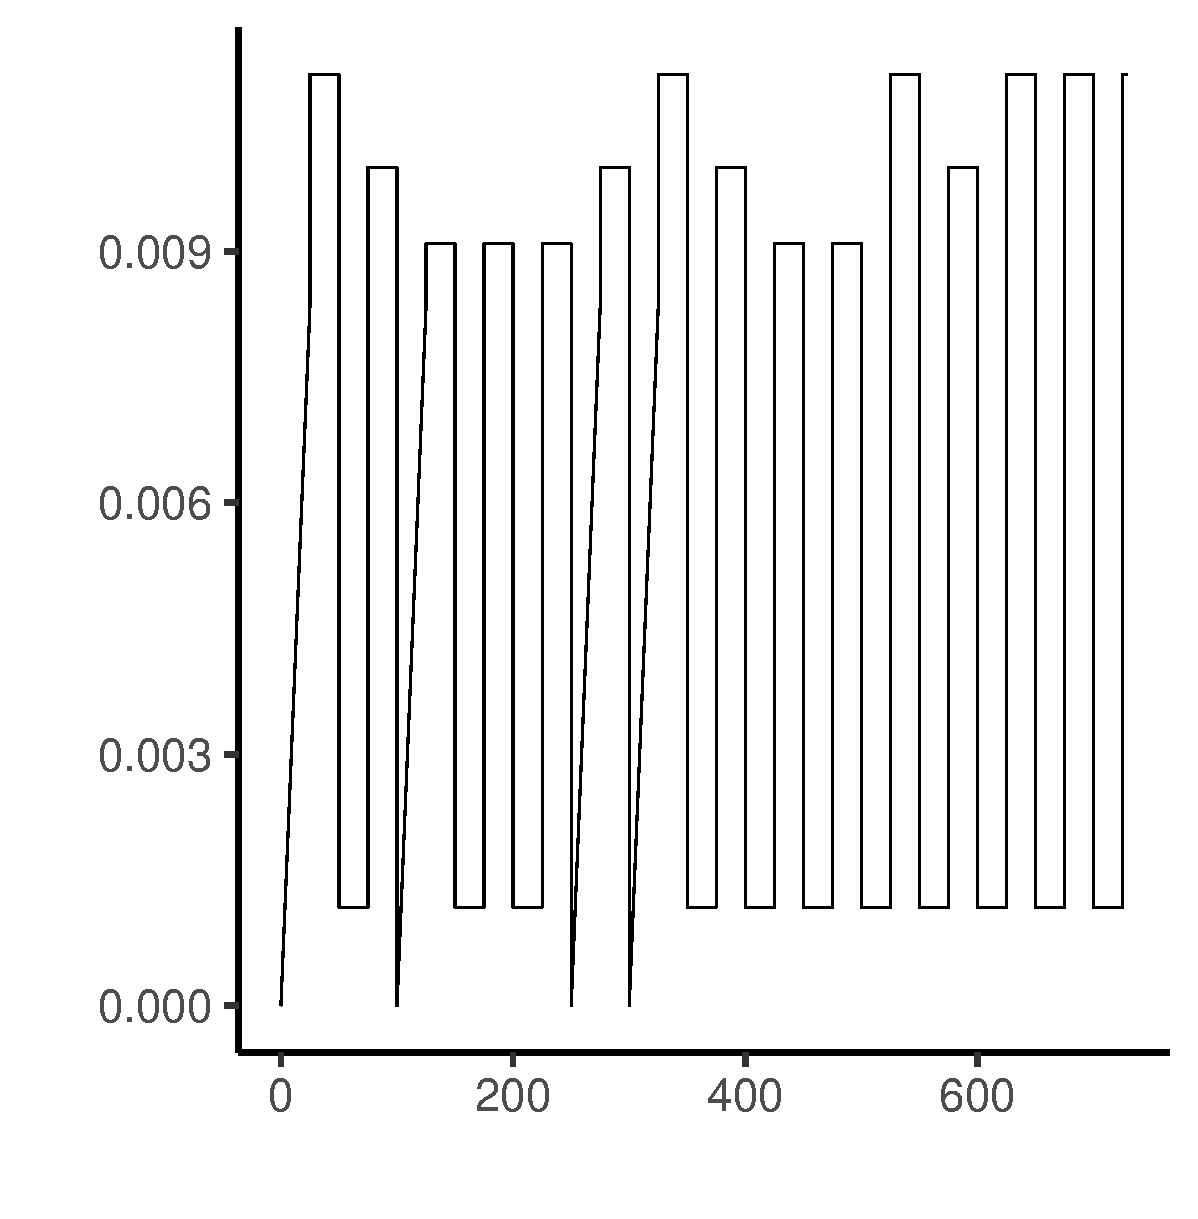
\includegraphics[width=0.55\textwidth,height=1.3in]{sim_base}
\end{figure}
\pause
\item For simplicity, we assume the linear predictor is $\eta_i = \gamma(u_i) + \epsilon_i$, with the true function $\gamma(u) = 1.5[\text{sin}(0.8u)+1]$. All the $u_i$ are independently generated from $\text{unif}[-6,6]$. 
\end{itemize}
\end{frame}

\begin{frame}
\begin{itemize}
\item Among these 400 observations, we randomly censored 80 of them. The covariate $u$ is discretized into 50 disjoint and equally-spaced bins.
\pause
\item We then implemented the RW2 smoothing using both our method and INLA. In both cases, the variance parameter $\sigma_u$ is set to have a PC prior such that $\textbf{P}(\sigma_u > 2.5) = 0.5$ \citep{pcprior}.
\pause
\item For the implementation of INLA, we used its default setting, which is to use a first-order random walk model for the baseline hazard. 
\pause
\item The results are summarized as the plot at the next page.
\end{itemize}
\end{frame}

\begin{frame}
\begin{figure}
\centering
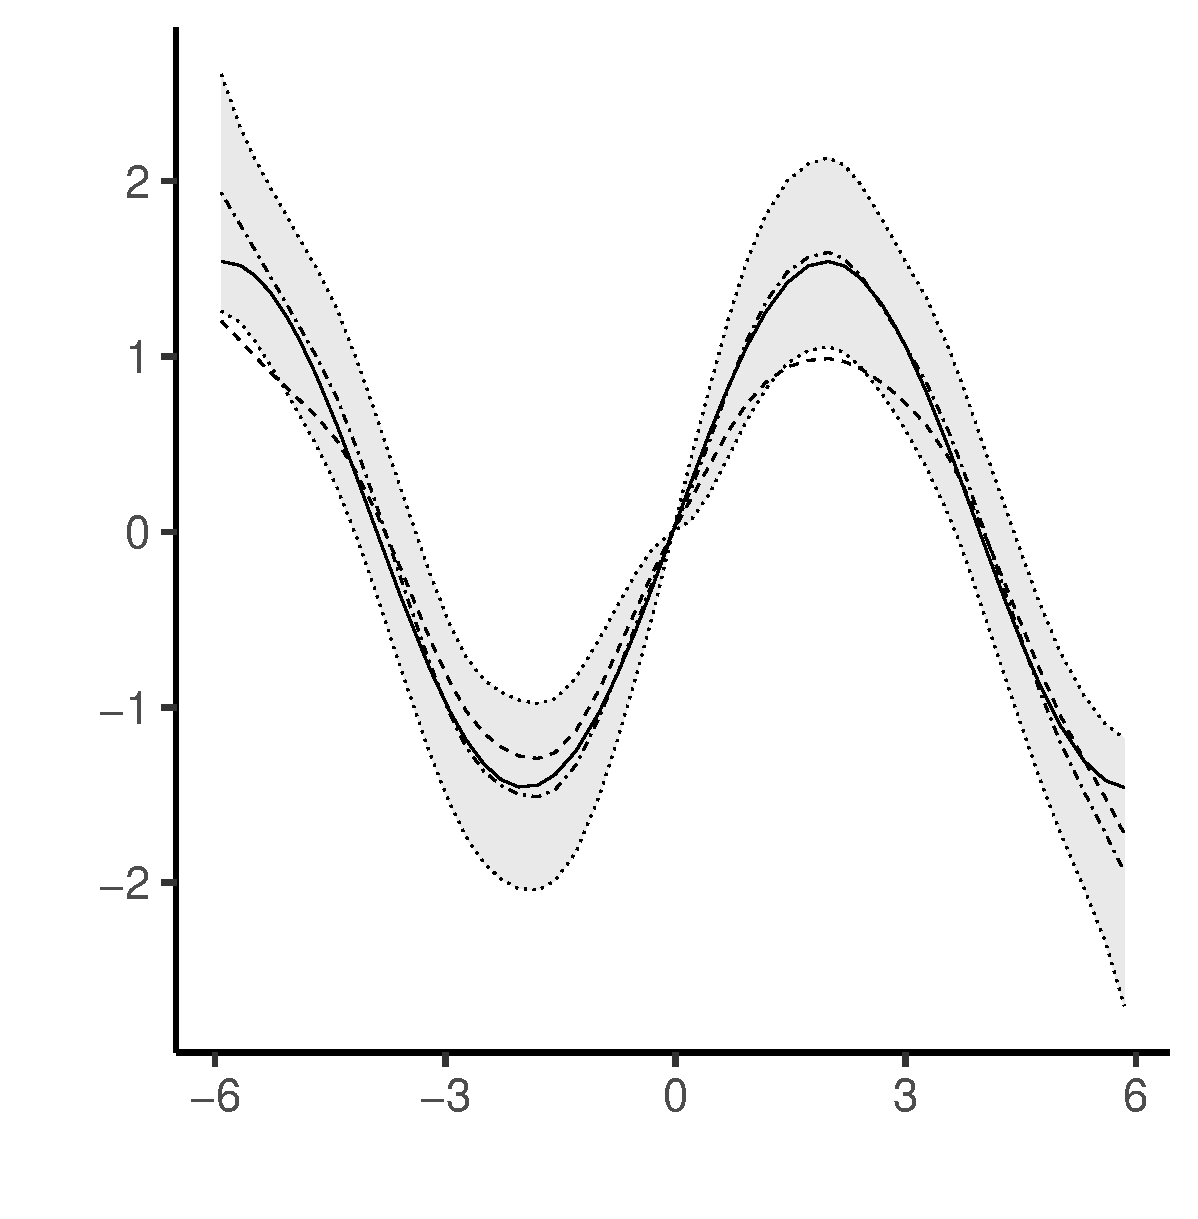
\includegraphics[width=0.75\textwidth,height=2.5in]{SmoothingSim_FinalPlot}
\caption{ True risk function (---); posterior mean (- $\cdot$ -) and $95\%$ credible interval ($\cdots$) using proposed method; posterior mean using INLA (- - -).}
\end{figure}
\end{frame}


\subsection{Applications for Leukaemia Data}
\begin{frame}
\cite{inlacoxph} analyzed the Leukaemia data set using INLA (therefore, full-likelihood). The dataset contains information from 1043 independent adult leukaemia patients, with 16 percent of observations right-censored. Specifically, the main interest is to quantify the relationship between survival rate of leukaemia patients with the Townsend deprivation index (\texttt{tpi}) corresponding to the patient's location, conditional on the \texttt{age} of the patient, the count of white blood cells at diagnosis (\texttt{wbc}) and \texttt{sex} of the patient.
\end{frame}

\begin{frame}
\begin{itemize}
\item The effects of \texttt{age}, \texttt{wbc} and \texttt{sex} were modelled linearly.Prior distributions $\beta \stackrel{iid}{\sim} \text{N}(0, 0.001^{-1})$, were used for the linear effects.
\pause
\item The \texttt{tpi} was discretized into 50 equally spaced bins and modelled as a semi-parametric (smoothing) effect. The semi-parametric effects $\Gamma = \{\gamma(\texttt{tpi}_1), \cdots, \gamma(\texttt{tpi}_{50})\}$ were modelled using the RW2 model with the reference constraint $\gamma(0) = 0$.
\pause
\item The single variance parameter $\sigma$ was given a PC prior such that $\text{P}(\sigma > 2) = 0.5$. 
\end{itemize}
\end{frame}

\begin{frame}
\begin{figure}
\centering
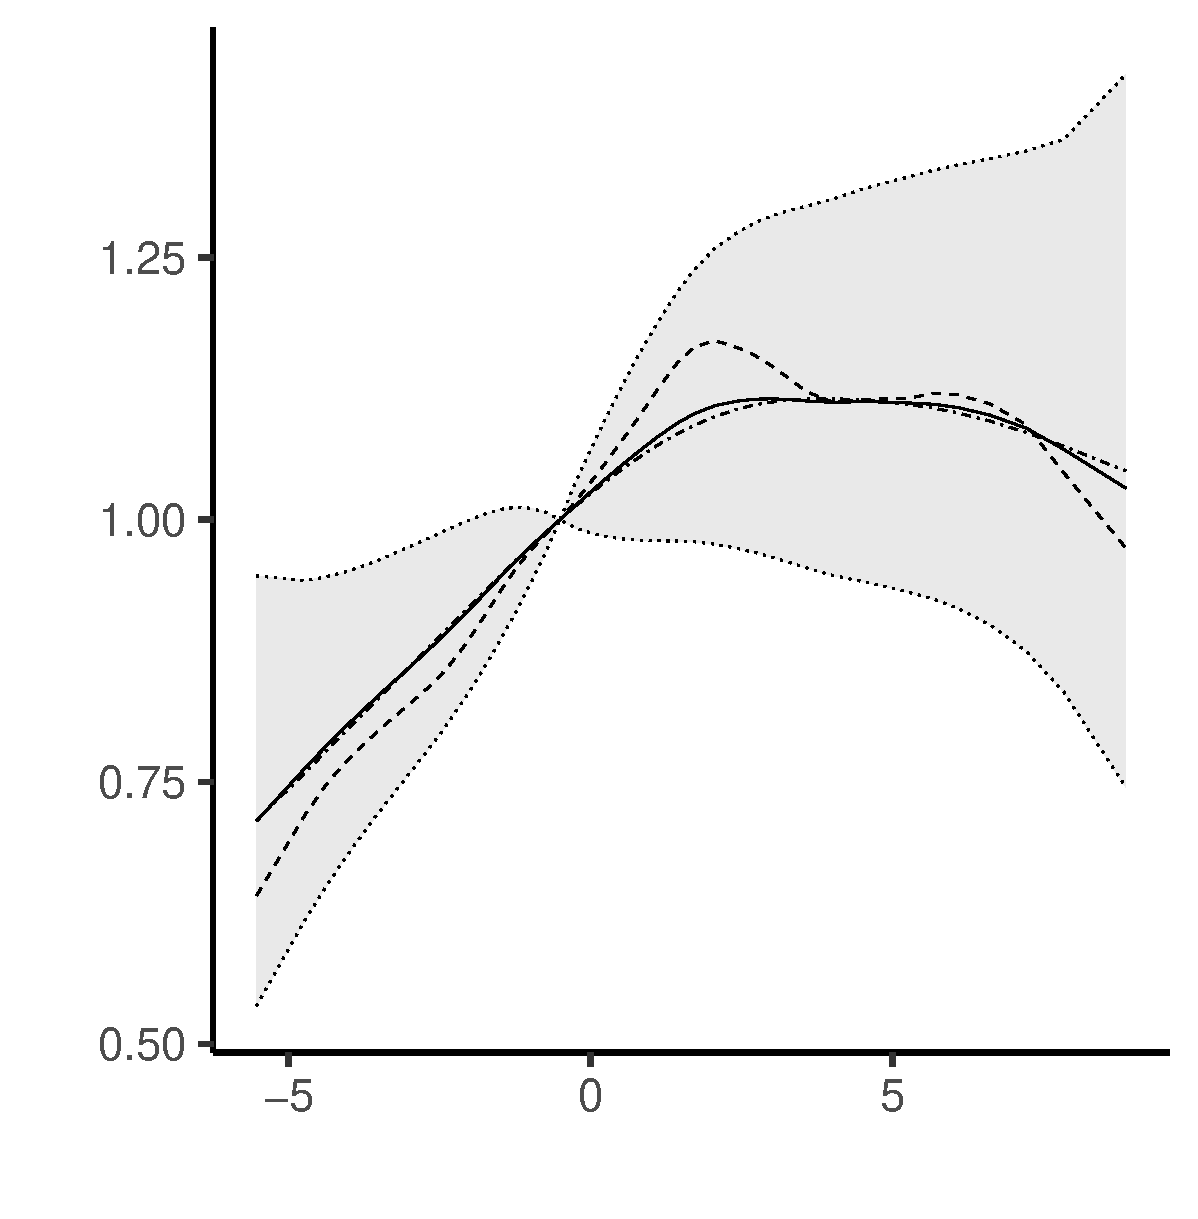
\includegraphics[width=0.45\textwidth,height=2.1in]{leuk_FinalPlot}
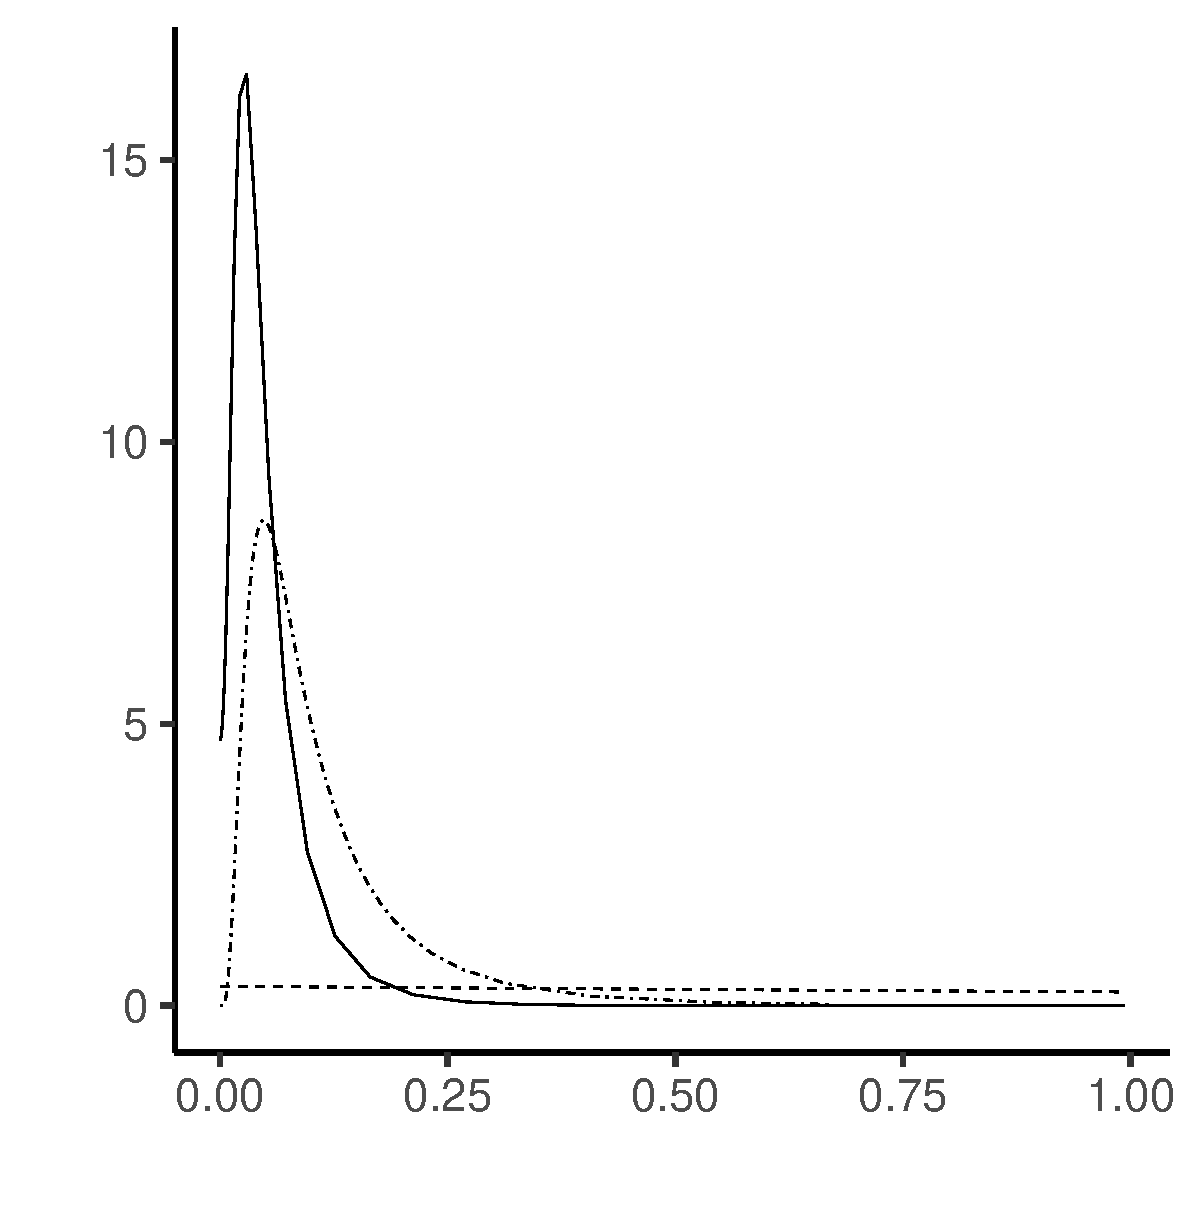
\includegraphics[width=0.45\textwidth,height=2.1in]{Leuk_PosterSigma}
\caption{(a): posterior mean (---) and $95\%$ credible interval ($\cdots$) using our method, posterior mean using INLA (- - -), and the result of fitting a GAM (- $\cdot$ -). (b): prior (- - -) and approximate posterior distribution for $\sigma$ using our method (---) and INLA (- $\cdot$ -).}
\end{figure}
\end{frame}

\section{Summary and Possible Extension}
\begin{frame}
\begin{itemize}
\item We introduce an approximate Bayesian inference method for Cox Proportional Hazard model with $\textbf{partial likelihood}$.
\pause
\item Because of the partial likelihood it used, the method does not have restriction on the form of baseline hazard function.
\pause
\item The proposed method allows the inference of semi-parametric smoothing effect, that is is not sensitive to the number and placement of bins.
\pause
\item The proposed method also allows observations to be correlated within subject (random intercept for subjects).
\pause
\item Compared to traditional frequentist's method, Bayesian inference provided model-based estimation and uncertainty
qualification.
\pause
\item Due to the stable and fast optimization algorithm (quasi-Newton method),  computations are $\textbf{fast}$ for small to median sized data set.
\end{itemize}
\end{frame}

\begin{frame}
\begin{itemize}
\item More types of effects? For example: Spatial effect, temporal effect ... 
\pause
Need to include other covariance structure.
\pause
\item More types of censoring? For example, besides traditional right-censoring, we can have: left-censoring, interval-censoring, left-truncations ... 
\pause
Need to modify the partial likelihood function. 
\pause
\item The method does not work efficient for data set that has very large size, as the computational cost grows as $O(n^2)$ (The fully dense Hessian matrix still needs to be evaluated at each maximum).
\end{itemize}
\end{frame}

\begin{frame}
\bibliography{refs}
\bibliographystyle{chicago}
\end{frame}


\end{document}